\section{Background \& Motivation}
\label{sec:background_motivation}
\subsection{The EVM Execution Model}
\begin{figure}[!htbp]
\centering
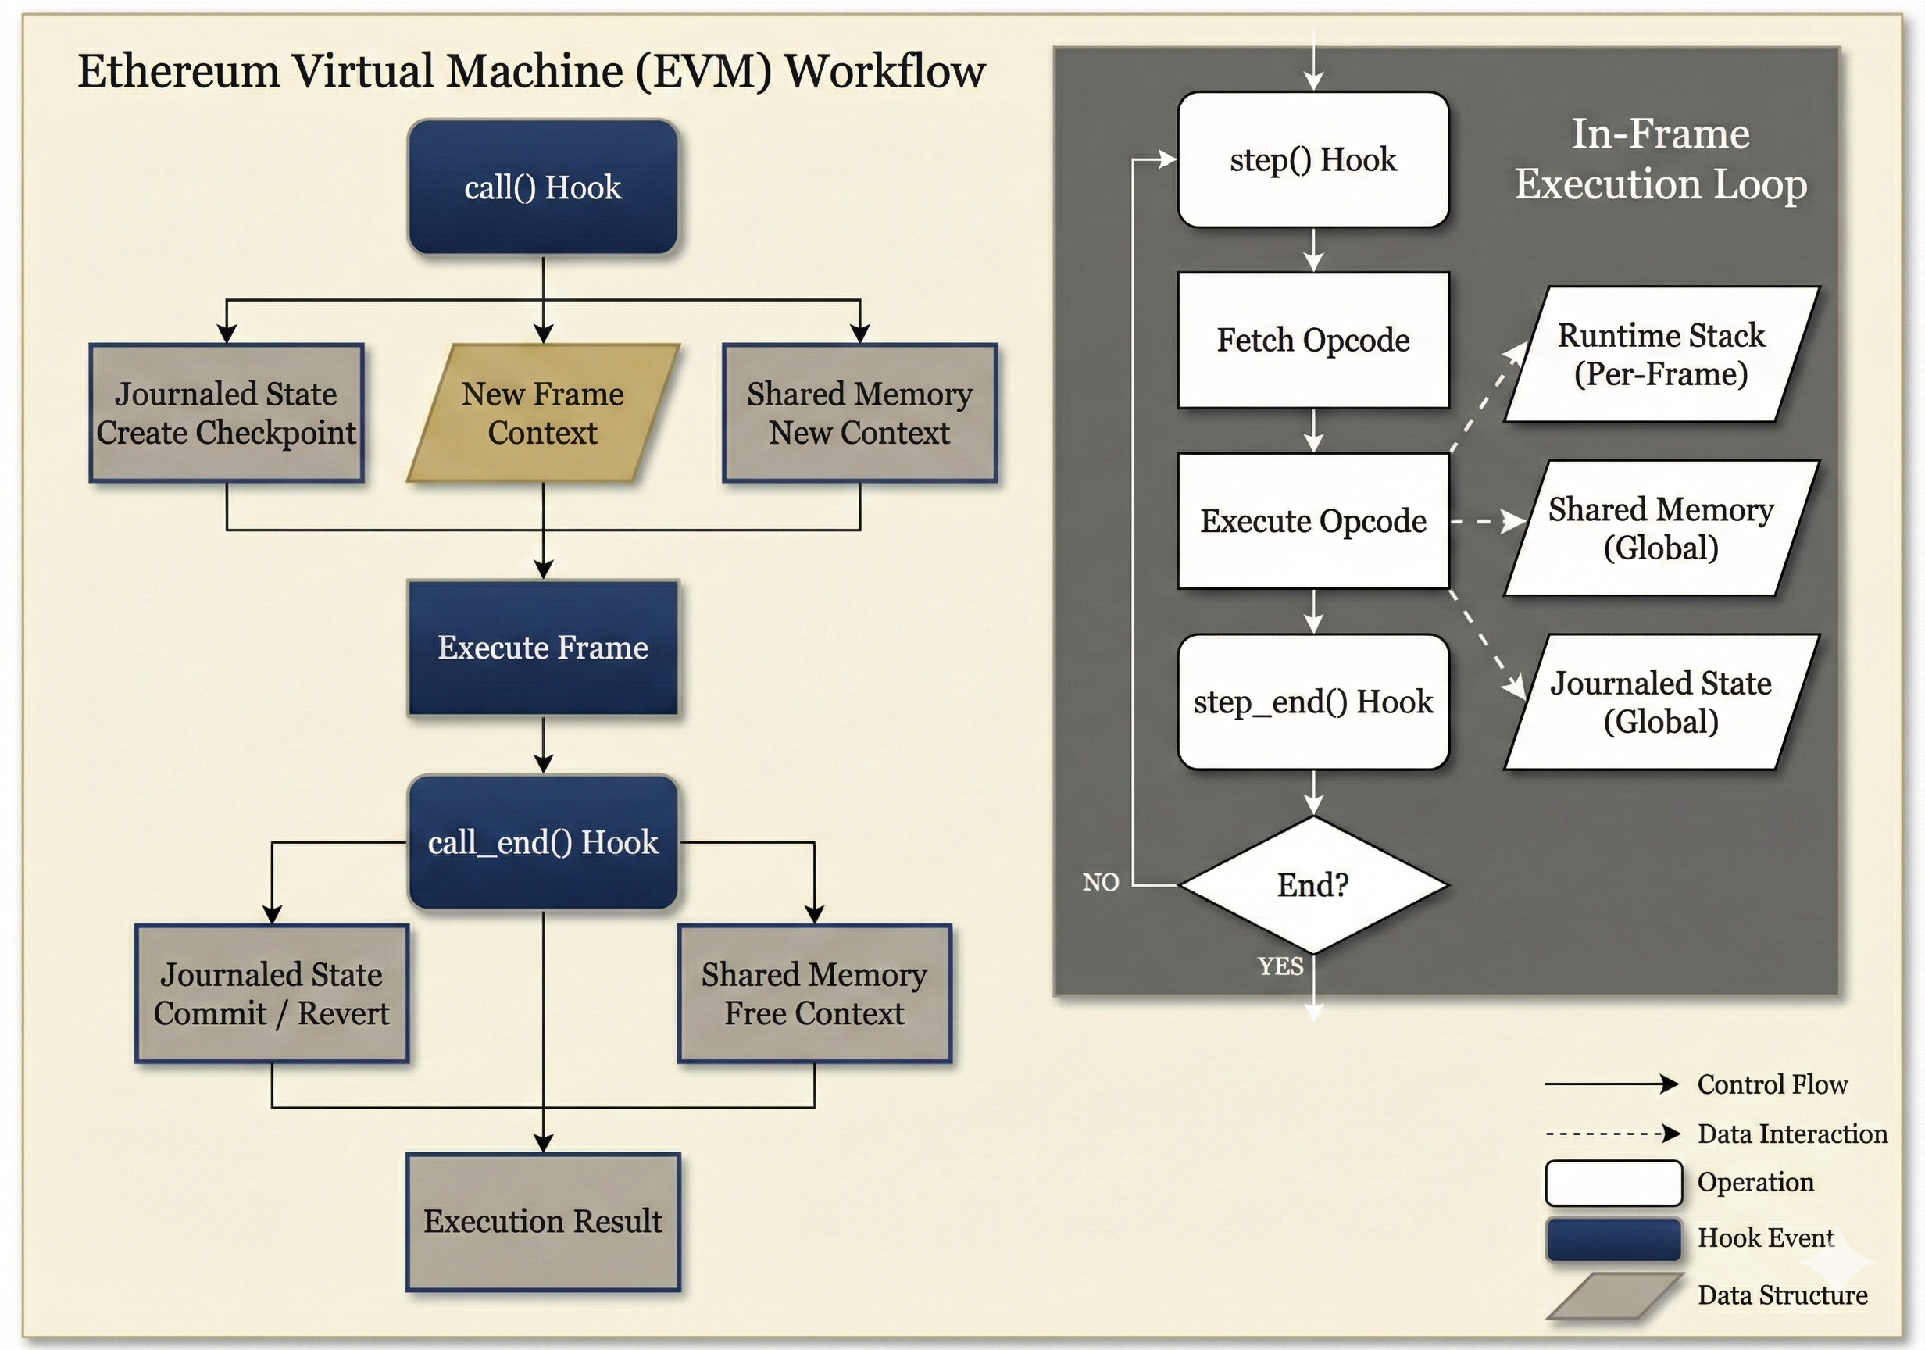
\includegraphics[width=\columnwidth]{raw-figures/EVM.drawio.pdf}
\caption{The EVM execution workflow. The process is partitioned into a high-level frame management lifecycle (left) and a low-level, per-opcode execution loop (right).}
\label{fig:evm-workflow}
\end{figure}

The EVM operates as a quasi-Turing-complete stack machine~\cite{ethereum}. Unlike register-based architectures, the EVM performs all computations on a transient runtime stack using specific manipulation instructions such as DUP and SWAP to manage operand placement. This design necessitates frequent stack operations that incur significant execution overhead.

Execution is compartmentalized into a hierarchy of call frames. Each frame maintains an isolated memory context and stack while sharing persistent storage access with other frames in the transaction. Resource consumption is metered via Gas, which functions as both a validator incentive and a security mechanism against denial-of-service attacks. Gas costs fall into two distinct categories. Static costs are fixed at compile time for computational operations. Dynamic costs depend on runtime states such as memory expansion or storage access frequency. This distinction enables optimization strategies that aggregate static costs while delegating dynamic accounting to the native handling logic.

Crucially, the EVM specification includes a standard hook mechanism to facilitate debugging and tracing. As illustrated in Figure~\ref{fig:evm-workflow}, this interface triggers events at key lifecycle points such as opcode execution and frame transitions. This design enables external components to passively observe execution states and capture data dependencies without requiring invasive modifications to the core interpreter logic.

\subsection{Ethereum Node Workloads}
The Ethereum network depends on node archetypes that exhibit divergent operational characteristics~\cite{eth-nodes-and-clients}. Full nodes operate within fixed block intervals and prioritize the low-latency processing of unpredictable transactions to ensure consensus stability. In contrast, archive nodes maintain the comprehensive ledger history and emphasize execution throughput to facilitate the bulk re-execution of historical states~\cite{geth-sync-modes, eth-archive-node}. This operational dichotomy introduces a dual challenge of optimizing for real-time responsiveness while simultaneously accommodating high-volume historical processing~\cite{feng2024slimarchive}.

\subsection{The Performance Paradox}
% require \usepackage{booktabs}
\begin{table}[t]
\centering
\caption{Performance degradation of path-driven optimization on modern EVMs. 
Measurements on Uniswap V2 swap (1-hop) demonstrate that artifact overhead 
dominates when baseline execution is fast.}
\label{tab:motivation-overhead}
\small
\resizebox{\columnwidth}{!}{%
\begin{tabular}{llrrr}
\toprule
\textbf{System} & \textbf{Client} & \textbf{Latency} & \textbf{Speedup} & \textbf{Artifact} \\
 & & \textbf{(µs)} & \textbf{(×)} & \textbf{(KB)} \\
\midrule
Native          & Geth         & 398.4   & 1.0×    & --    \\
Forerunner      & Geth         & 68.1    & 5.8×    & 910   \\
\midrule
Native          & Revm         & 62.0    & 1.0×    & --    \\
Forerunner      & Revm         & 39.2    & 1.6×    & 663   \\
\midrule
\textbf{Helios} & \textbf{Revm} & \textbf{31.0} & \textbf{2.0×} & \textbf{70} \\
\bottomrule
\end{tabular}%
}
\end{table}

Contract-driven optimization, exemplified by JIT compilation, faces two critical limitations in permissionless blockchains. First, it introduces an attack surface known as "JIT bombs" where attackers construct pathological code patterns, such as deeply nested conditional branches, to trigger exponential compilation complexity. This computational asymmetry allows malicious actors to exhaust validator CPU resources via low-gas transactions and constitutes a Denial-of-Service vector~\cite{revmc,monad,evmjit,bnbjit,JITBomb}. 

Second, strict gas-semantic equivalence is a fundamental economic and functional constraint. Any systematic deviation from the canonical gas schedule results in incorrect validator compensation, distorting market incentives and impeding the deployment of production clients. Aggressive compiler optimizations like instruction reordering often alter the observable gas schedule, making consensus preservation difficult without complex runtime compensation. Consequently, path-driven optimization emerges as a safer paradigm by inherently bounding optimization costs to the actual execution trace.

However, existing path-driven schemes encounter a scalability barrier on modern EVM clients, a phenomenon we term the \textit{Performance Paradox}. On slower engines like Geth~\cite{geth}, transaction execution dominates end-to-end latency, rendering the additional instrumentation cost negligible. Conversely, on highly optimized engines like Revm~\cite{revm}, the critical path shifts as execution becomes inexpensive, causing auxiliary tasks such as tracing and artifact management to become the primary bottleneck. Table~\ref{tab:motivation-overhead} demonstrates this shift using a Uniswap V2 swap~\cite{uniswapv2}. A prior path-driven system~\cite{forerunner} achieves a 5.8$\times$ speedup on Geth but only 1.6$\times$ on Revm. Two factors explain this performance degradation. First, synchronous tracing dominates the critical path. On Revm, tracing a transaction is approximately six times slower than native execution and nearly ten times slower than optimized execution, effectively negating the potential benefits. Second, artifact management incurs substantial fixed costs. Loading and parsing a $663\,\text{KB}$ artifact to accelerate a task finishing in tens of microseconds introduces I/O latency that does not scale with the underlying execution time. These constraints necessitate two architectural shifts: replacing synchronous tracing with asynchronous optimization off the critical path and substituting large artifacts with lightweight traces to minimize data volume.

\subsection{The Granularity Mismatch}
\begin{figure}[b]
\centering
\includegraphics[width=\columnwidth]{raw-figures/pareto_cumulative.pdf}
\caption{Path locality in EVM execution follows an extreme Pareto distribution: the top 1\% of unique paths account for 70\% of frame executions (5,000 mainnet blocks). The shaded region shows deviation from uniform distribution.}
\label{fig:pareto-cumulative}
\end{figure}

Beyond tracing overhead, existing strategies predominantly employ transaction-level caching~\cite{forerunner,seer,parallelEvm}. This approach treats the entire transaction execution trace as the atomic unit of optimization. It faces a combinatorial challenge because slight variations in the sequence of internal contract calls render the entire cached artifact invalid. This dependency enforces a "use-once-discard" lifecycle that limits reuse potential.

In contrast, our analysis of Ethereum mainnet workloads reveals significant redundancy at the finer frame granularity. As shown in Figure~\ref{fig:pareto-cumulative}, the distribution of unique frame paths follows a Pareto principle where the top 1\% of paths account for over 70\% of total executions. This disparity indicates that while unique transaction combinations are vast, the individual contract calls function as repetitive building blocks. Shifting the optimization unit from transactions to frames aligns the caching strategy with this inherent locality and enables the amortization of compilation costs across thousands of invocations.

\subsection{Design Implications} 
The preceding analysis suggests three architectural principles for a high-performance EVM accelerator. First, the distinction between static and dynamic gas costs motivates a hybrid execution model. Optimizing only static instructions while delegating dynamic operations to the native handling ensures gas-semantic equivalence by construction. Second, the Performance Paradox necessitates asynchronous lightweight tracing and optimization. Decoupling these tasks from the critical path limits I/O overhead and preserves baseline execution speed. Third, the pronounced path locality implies the need for frame-level persistent caching. This granularity enables compositional artifact reuse across diverse transactions, overcoming the limitations of transaction-level approaches. These principles collectively inform the design of Helios.